% !TeX program = xelatex
% !TeX encoding = UTF-8
% Poster: AI_TLfanclub at VLSP 2026 ViTNumChart
% Build: latexmk -xelatex poster.tex
\documentclass[a1paper,portrait,movebody=8.4mm]{baposter}

\usepackage{amsmath}
\usepackage{fontspec}
\usepackage{unicode-math}
\setsansfont{FiraSans}[
  Extension=.otf, UprightFont=*-Regular, BoldFont=*-Medium,
  ItalicFont=*-Italic, BoldItalicFont=*-MediumItalic]
\newfontfamily\lightfont{FiraSans}[Extension=.otf, UprightFont=*-Light, BoldFont=*-Regular]
\setmonofont{FiraMono}[Extension=.otf, UprightFont=*-Regular, BoldFont=*-Medium, Scale=0.92]
\setmathfont{FiraMath-Regular.otf}
\renewcommand{\familydefault}{\sfdefault}
\usepackage[english]{babel}

\usepackage{booktabs}
\usepackage{paralist}
\usepackage{xcolor}
\usepackage{pgfplots}
\pgfplotsset{compat=1.18, every axis x label/.append style={yshift=-3pt}}
\usetikzlibrary{arrows.meta,positioning,calc}

% ---- colours: one accent, the rest neutral --------------------------------
\definecolor{accent}{RGB}{165,28,48}     % HUST red, slightly deepened
\definecolor{ink}{RGB}{28,30,34}
\definecolor{muted}{RGB}{95,99,107}
\colorlet{rulegray}{black!18}
\colorlet{hustred}{accent}               % used by the figure files

% ---- section headers: dark text over a thin accent rule -------------------
\makeatletter
\renewcommand{\baposter@box@headerdrawtext@rectangle}[1]{%
  \path (\baposter@box@name nw) +(0pt,-0.55\baposter@box@@boxheaderheight)
        node[anchor=west, inner xsep=0pt, inner ysep=0pt] {#1};%
  \draw[accent, line width=1.6pt] (\baposter@box@name tnw) -- (\baposter@box@name tne);%
}
\makeatother
\newcommand{\secno}[1]{\textcolor{accent}{#1}\hspace{0.55em}}

% ---- helpers ------------------------------------------------------------
\newcommand{\progfont}[1]{{\ttfamily #1}}
% Vietnamese labels inside programs: FiraMono lacks some precomposed glyphs (e.g. U+1EA7)
\newcommand{\vnlabel}[1]{{\sffamily #1}}
\newcommand{\pp}{\,pp}
\newcommand{\note}[1]{{\small\color{muted}#1}}
\newcommand{\notepar}[1]{{\small\color{muted}\raggedright #1\par}}

% a key figure set in type: number, then a caption underneath
\newcommand{\keyfig}[2]{%
  {\lightfont\fontsize{24}{26}\selectfont\color{accent}#1}\\[4pt]
  {\raggedright\footnotesize\color{ink}#2\par}}

\setlength{\parindent}{0pt}
\setlength{\parskip}{4pt}

\begin{document}
\color{ink}

\begin{poster}{
    grid=false,
    columns=3,
    colspacing=1.1em,
    headerheight=0.095\textheight,
    eyecatcher=true,
    background=none,
    borderColor=white,
    headerColorOne=white,
    headerColorTwo=white,
    headerFontColor=ink,
    boxColorOne=white,
    headershape=rectangle,
    headershade=plain,
    headerfont=\sffamily\bfseries\large,
    boxheaderheight=1.95em,
    boxpadding=0.35em,
    textborder=none,
    headerborder=none,
    boxshade=none,
    linewidth=0pt,
  }
  % ---- eye catcher: HUST logo ----------------------------------------------
  {
\includegraphics[height=0.075\textheight]{logos/hust_crop.jpg}}
  % ---- title ------------------------------------------------------------------
  {\color{ink}\fontsize{27}{32}\selectfont\bfseries
    AI\_TLfanclub at VLSP 2026 ViTNumChart:\\[2pt]
    {\fontsize{20}{25}\selectfont\mdseries Voting over Fine-Tuned Small Multimodal Program Writers,\\ with an Analysis of Single-Writer Errors}}
  % ---- authors ----------------------------------------------------------------
  {\vspace{0.4em}\large
    Do Thanh Duc \quad Vu Viet Anh \quad Nguyen Nhat Minh\\[2pt]
    {\normalsize\color{muted} School of Information and Communication Technology, Hanoi University of Science and Technology}\\[1pt]
    {\small\color{muted}\ttfamily \{duc.dt242095m, anh.vv251047m, minh.nn252184m\}@sis.hust.edu.vn}}
  % ---- right logo: VLSP 2026 -------------------------------------------------
  {
\includegraphics[height=0.078\textheight]{logos/vlsp2026.png}}

%==============================================================================
\headerbox{}{name=glance,column=0,row=0,span=3}{
  \noindent\makebox[\linewidth][c]{\color{rulegray}\rule{\dimexpr\linewidth+0.7em\relax}{0.8pt}}\par\vspace{1.5mm}
  \begin{minipage}[c]{0.15\linewidth}
    \keyfig{1st of 9}{teams on the private\\leaderboard}
  \end{minipage}%
  {\color{rulegray}\vrule width 0.8pt height 7mm depth 7mm}\hspace{1.2em}%
  \begin{minipage}[c]{0.17\linewidth}
    \keyfig{0.7917}{Program Accuracy, private test\\{\color{muted}runner-up 0.7866}}
  \end{minipage}%
  {\color{rulegray}\vrule width 0.8pt height 7mm depth 7mm}\hspace{1.2em}%
  \begin{minipage}[c]{0.61\linewidth}
    A base \textbf{Qwen3-VL-4B} transcribes every chart, \textbf{26 LoRA-tuned Qwen3.5-4B} writers each write one program, and a \textbf{plurality vote} over their canonical programs picks the answer. Every model has at most 8B parameters.\\[3pt]
    \textcolor{accent}{\textbf{1}}\enspace Combining writers that \emph{differ} helps more than decoding one writer more often.\\[1pt]
    \textcolor{accent}{\textbf{2}}\enspace A single writer's errors start early, are shared across writers, and resisted every training remedy we tried.
  \end{minipage}
  \par\vspace{1.5mm}\noindent\makebox[\linewidth][c]{\color{rulegray}\rule{\dimexpr\linewidth+0.7em\relax}{0.8pt}}
}

\headerbox{\secno{1}Task: ViTNumChart}{name=task,column=0,below=glance}{
  Answer a numerical question over a \textbf{Vietnamese financial report} (paragraphs, HTML tables, chart images) by writing a \textbf{reasoning program}. Arithmetic steps (\texttt{add}, \texttt{subtract}, \texttt{multiply}, \texttt{divide}, \texttt{greater}) take numbers or references \texttt{\#k}; retrieval steps \texttt{table\_op}, \texttt{chart\_op} copy labels from the document.

  \vspace{3mm}
  % Constructed task example (Fig. 1 of the paper), redrawn.
\begin{tikzpicture}[
    panel/.style={draw=black!25, fill=white, line width=0.6pt, inner sep=5pt},
    lab/.style={font=\scriptsize\bfseries\color{muted}, anchor=south west, inner sep=1.5pt},
  ]
  % ---- input chart --------------------------------------------------------
  \node[panel, anchor=north west] (chart) at (0,0) {%
    \begin{tikzpicture}
      \begin{axis}[
          width=3.9cm, height=3.6cm, scale only axis=false,
          ybar, bar width=13pt,
          ymin=0, ymax=1850,
          symbolic x coords={2023,2024}, xtick=data,
          enlarge x limits=0.6,
          axis lines*=left, ytick=\empty,
          tick label style={font=\scriptsize},
          nodes near coords, nodes near coords style={font=\scriptsize, /pgf/number format/set thousands separator={.}},
          title={\scriptsize Doanh thu thuần (tỷ đồng)},
          title style={yshift=-5pt},
        ]
        \addplot[fill=black!50, draw=none] coordinates {(2023,1310) (2024,1520)};
      \end{axis}
    \end{tikzpicture}};
  \node[lab] at (chart.north west) {IMAGE 1};

  % ---- question -------------------------------------------------------------
  \path (chart.north east) ++(3mm,0) coordinate (qanchor);
  \node[panel, anchor=north west, font=\small, minimum height=0pt,
        text width=\dimexpr\linewidth-4.45cm\relax] (q) at (qanchor) {%
    \textbf{Question} {\scriptsize\color{muted}(translated)}\\[1pt]
    By how much did net revenue change from 2023 to 2024?\\[4pt]
    {\footnotesize\color{muted}Context: report paragraphs, HTML tables, up to 13 images in the public test}};
  \node[lab] at (q.north west) {INPUT};

  % ---- programs -----------------------------------------------------------
  \node[panel, anchor=north west, text width=\dimexpr\linewidth-11pt\relax, font=\footnotesize] (prog) at ([yshift=-6mm]chart.south west) {%
    \renewcommand{\arraystretch}{1.25}%
    \begin{tabular}{@{}l@{\hspace{6pt}}p{\dimexpr\linewidth-38pt\relax}@{}}
      {\scriptsize\bfseries gold} & \progfont{chart\_at(Image 1; \vnlabel{Doanh thu thuần}; 2024; none); chart\_at(Image 1; \vnlabel{Doanh thu thuần}; 2023; none); \mbox{subtract}(\#0; \#1)}\\[2pt]
      {\scriptsize\bfseries\color{accent}error} & \progfont{chart\_at(Image 1; \textcolor{accent}{\underline{Doanh thu}}; 2024; none); \dots}\newline{\scriptsize\color{muted}label not as printed on the chart}\\[2pt]
      {\scriptsize\bfseries\color{accent}error} & \progfont{subtract(\textcolor{accent}{\underline{1520}}; \textcolor{accent}{\underline{1310}})}\newline{\scriptsize\color{muted}right value, but typed from the bars}\\
    \end{tabular}};
  \node[lab] at (prog.north west) {OUTPUT: A PROGRAM, SCORED BY PROGRAM ACCURACY (PA)};
\end{tikzpicture}

}

\headerbox{\secno{4}System}{name=system,column=0,span=3,below=task}{
  \vspace{2mm}
  \begin{center}
    \resizebox{\linewidth}{!}{% Inference pipeline (Fig. 2 of the paper), redrawn.
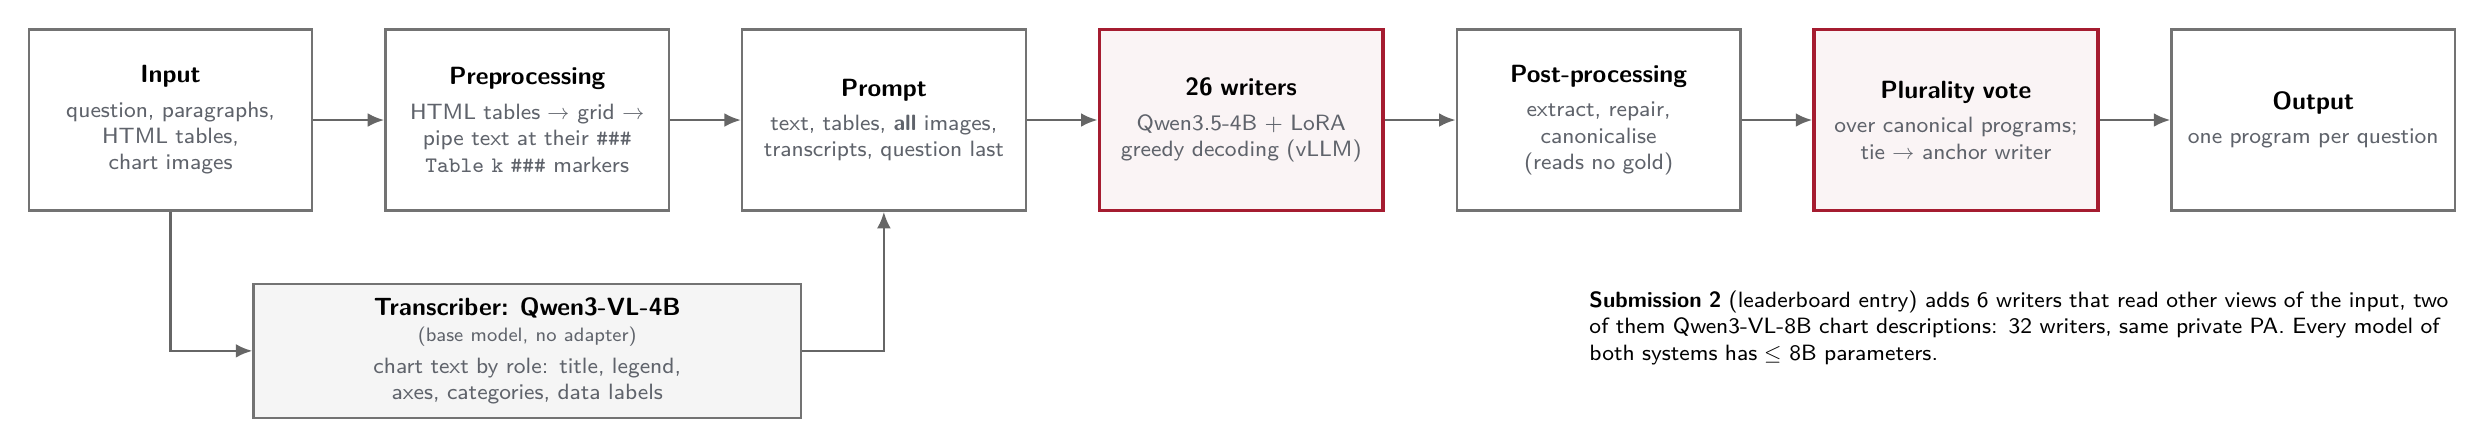
\begin{tikzpicture}[
    node distance=9mm,
    stage/.style={draw=black!55, fill=white, line width=0.8pt,
                  text width=3.25cm, minimum height=2.3cm, align=center, inner sep=5pt, font=\footnotesize,
                  execute at begin node={\hyphenpenalty=10000\exhyphenpenalty=10000}},
    key/.style={stage, draw=accent, line width=1.3pt, fill=accent!5},
    arr/.style={-{Latex[length=6pt,width=5pt]}, line width=1pt, color=black!60},
  ]
  \node[stage] (in) {{\small\bfseries Input}\\[3pt]{\color{muted}question, paragraphs, HTML tables, chart images}};
  \node[stage, right=of in] (pre) {{\small\bfseries Preprocessing}\\[3pt]{\color{muted}HTML tables $\to$ grid $\to$ pipe text at their \texttt{\#\#\# Table k \#\#\#} markers}};
  \node[stage, right=of pre] (prompt) {{\small\bfseries Prompt}\\[3pt]{\color{muted}text, tables, \textbf{all} images, transcripts, question last}};
  \node[key, right=of prompt] (wr) {{\small\bfseries 26 writers}\\[3pt]{\color{muted}Qwen3.5-4B + LoRA\\greedy decoding (vLLM)}};
  \node[stage, right=of wr] (post) {{\small\bfseries Post-processing}\\[3pt]{\color{muted}extract, repair, canonicalise (reads no gold)}};
  \node[key, right=of post] (vote) {{\small\bfseries Plurality vote}\\[3pt]{\color{muted}over canonical programs; tie $\to$ anchor writer}};
  \node[stage, right=of vote] (out) {{\small\bfseries Output}\\[3pt]{\color{muted}one program per question}};

  \node[stage, text width=6.6cm, minimum height=1.3cm, anchor=north, fill=black!4]
     (tr) at ([yshift=-9mm]pre.south)
     {{\small\bfseries Transcriber: \mbox{Qwen3-VL-4B}} {\scriptsize\color{muted}(base model, no adapter)}\\[2pt]{\color{muted}chart text by role: title, legend, axes, categories, data labels}};

  \draw[arr] (in) -- (pre);
  \draw[arr] (pre) -- (prompt);
  \draw[arr] (prompt) -- (wr);
  \draw[arr] (wr) -- (post);
  \draw[arr] (post) -- (vote);
  \draw[arr] (vote) -- (out);
  \draw[arr] (in.south) |- (tr.west);
  \draw[arr] (tr.east) -| (prompt.south);

  \node[font=\footnotesize, text width=11cm, align=left, anchor=north east, inner sep=0pt]
    at ([yshift=-10mm]out.south east)
    {\textbf{Submission 2} (leaderboard entry) adds 6 writers that read other views of the input, two of them Qwen3-VL-8B chart descriptions: 32 writers, same private PA. Every model of both systems has $\le$ 8B parameters.};
\end{tikzpicture}
}
  \end{center}
}

\headerbox{\secno{2}Data and official results}{name=results,column=1,below=glance,above=system}{
  \begin{center}
  \small
  \begin{tabular}{@{}lccc@{}}
    \toprule
                    & Train & Public & Private \\
    \midrule
    Questions       & 1725  & 459    & 980 \\
    Documents       & 74    & 19     & 39 \\
    Distinct images & 187   & 61     & 83 \\
    Chart-step gold & 678   & 202    & -- \\
    \bottomrule
  \end{tabular}
  \end{center}
  \notepar{The public test is development data only and is never used for training.}

  \begin{center}
  \small
  \setlength{\tabcolsep}{4pt}
  \begin{tabular}{@{}lccc@{}}
    \toprule
    Submission & Public & \multicolumn{2}{c}{Private} \\
    \cmidrule(l){3-4}
               & strict & PA & EA \\
    \midrule
    1\enspace Vote, 26 writers    & 74.07 & \textbf{0.7917} & 0.8916\\
    2\enspace + views, 32 writers\textsuperscript{*} & 74.51 & \textbf{0.7917} & \textbf{0.8933}\\
    3\enspace Larger vote         & 74.51 & 0.79   & --\\
    4\enspace HTML-table writer   & 73.42 & 0.7711 & --\\
    \bottomrule
  \end{tabular}
  \end{center}
  \notepar{\textsuperscript{*}Leaderboard entry; private values as printed by the platform. EA (value) exceeds PA (program), consistent with errors in the program's \emph{form} (Box~10).}

  \smallskip
  \textbf{Accuracy by slice} \note{(public strict \%; members chosen on this set)}\par
  {\centering\small
  \begin{tabular}{@{}lrcc@{}}
    \toprule
    Slice & $n$ & Anchor & Vote \\
    \midrule
    Arithmetic only  & 182 & 76.4 & 81.3\\
    Table step       & 75  & 66.7 & 66.7\\
    Chart step       & 202 & 67.8 & 70.3\\
    Unseen structure & 43  & 11.6 & 20.9\\
    \bottomrule
  \end{tabular}\par}
}

\headerbox{\secno{3}Training the writers}{name=train,column=2,below=glance,above=system}{
  \begin{compactitem}
    \item Each training question becomes one chat example: the inference prompt, with the gold program as target.
    \item \textbf{LoRA} $r{=}32$, $\alpha{=}64$ on attention, MLP and Gated DeltaNet projections; vision tower frozen.
    \item lr $10^{-4}$, 3 epochs, bf16, prompts $\le$ 6{,}144 tokens.
    \item Median 0.87\,h per writer on one RTX 5090.
    \item Training prompts attach the gold images plus 1--2 distractor images; inference attaches \emph{every} image.
    \item Five document-level folds for cross-fitting; no external data.
  \end{compactitem}

  \medskip
  \textbf{The 26 vote members} \note{(submission 1)}\\[4pt]
  % Composition of the 26 vote members of submission 1 (Sec. 3.2 of the paper).
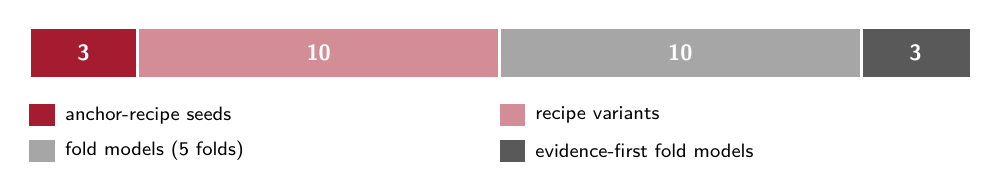
\begin{tikzpicture}[x=\dimexpr\linewidth/26-0.2pt\relax]
  \def\h{0.6}
  \fill[accent]       (0,0)  rectangle (3,\h);
  \fill[accent!50]    (3,0)  rectangle (13,\h);
  \fill[black!35]     (13,0) rectangle (23,\h);
  \fill[black!65]     (23,0) rectangle (26,\h);
  \foreach \a/\b/\n in {0/3/3, 3/13/10, 13/23/10, 23/26/3}{
    \node[font=\footnotesize\bfseries, white] at ({(\a+\b)/2},\h/2) {\n};
    \draw[white, line width=1.2pt] (\a,0) -- (\a,\h);
  }
  % legend in two rows
  \begin{scope}[every node/.style={font=\scriptsize, anchor=west, inner sep=1pt}]
    \fill[accent]       (0,-0.35)  rectangle ++(0.7,-0.28); \node at (0.9,-0.49)  {anchor-recipe seeds};
    \fill[accent!50]    (13,-0.35) rectangle ++(0.7,-0.28); \node at (13.9,-0.49) {recipe variants};
    \fill[black!35]     (0,-0.8)   rectangle ++(0.7,-0.28); \node at (0.9,-0.94)  {fold models (5 folds)};
    \fill[black!65]     (13,-0.8)  rectangle ++(0.7,-0.28); \node at (13.9,-0.94) {evidence-first fold models};
  \end{scope}
\end{tikzpicture}


  \notepar{All share backbone and prompt; they differ in target format, training folds, seed and objective, so that their \emph{errors} differ.}
}

\headerbox{\secno{6}Ablations and training remedies}{name=abl,column=1,below=system}{
  Public set, wild cluster bootstrap-t, Holm over 23 tests.\\
  \tikz[baseline=0pt]\fill[accent] (0,0) rectangle (6pt,6pt);\,survives Holm\qquad
  \tikz[baseline=0pt]\fill[black!45] (3pt,3pt) circle (3pt);\,not resolved

  \begin{center}% Forest plot of selected system ablations and remedies (Table 5 of the paper).
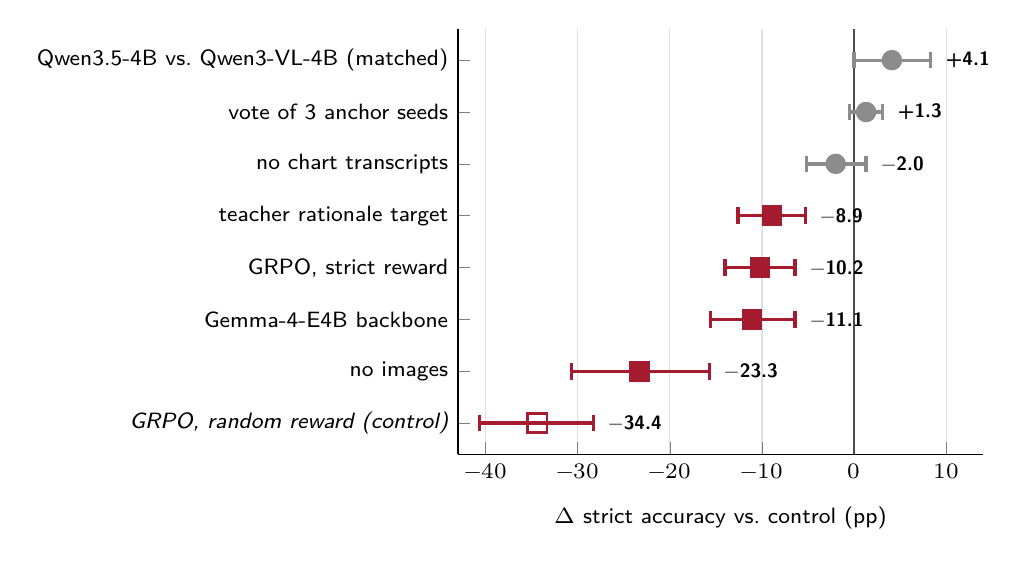
\begin{tikzpicture}
  \begin{axis}[
      width=0.55\linewidth, height=5.4cm, scale only axis,
      xmin=-43, xmax=14, clip=false,
      ymin=0.4, ymax=8.6, y dir=reverse,
      ytick={1,...,8},
      yticklabels={
        {Qwen3.5-4B vs.\ Qwen3-VL-4B (matched)},
        {vote of 3 anchor seeds},
        {no chart transcripts},
        {teacher rationale target},
        {GRPO, strict reward},
        {Gemma-4-E4B backbone},
        {no images},
        {\itshape GRPO, random reward (control)}},
      yticklabel style={font=\footnotesize, align=right},
      xtick={-40,-30,-20,-10,0,10},
      xlabel={$\Delta$ strict accuracy vs.\ control (pp)},
      xlabel style={font=\footnotesize},
      tick label style={font=\footnotesize},
      axis x line*=bottom, axis y line*=left,
      xmajorgrids, grid style={black!12},
      error bars/x dir=both, error bars/x explicit,
      error bars/error bar style={line width=1.2pt},
      error bars/error mark options={rotate=90, mark size=3pt, line width=1.2pt},
    ]
    \draw[black!70, line width=1pt] (axis cs:0,0.4) -- (axis cs:0,8.6);
    % not resolved after Holm
    \addplot[only marks, mark=*, mark size=3.5pt, black!45, error bars/error bar style={black!45, line width=1.2pt}] coordinates {
      (4.1,1)  += (4.2,0) -= (4.1,0)
      (1.3,2)  += (1.8,0) -= (1.8,0)
      (-2.0,3) += (3.3,0) -= (3.2,0)
    };
    % survives Holm
    \addplot[only marks, mark=square*, mark size=3.5pt, hustred] coordinates {
      (-8.9,4)  += (3.6,0) -= (3.7,0)
      (-10.2,5) += (3.8,0) -= (3.8,0)
      (-11.1,6) += (4.7,0) -= (4.5,0)
      (-23.3,7) += (7.6,0) -= (7.4,0)
    };
    \addplot[only marks, mark=square, mark size=3.5pt, hustred, line width=1pt] coordinates {
      (-34.4,8) += (6.1,0) -= (6.3,0)
    };
    \node[font=\scriptsize\bfseries, anchor=west, xshift=2pt] at (axis cs:8.3,1) {+4.1};
    \node[font=\scriptsize\bfseries, anchor=west, xshift=2pt] at (axis cs:3.1,2) {+1.3};
    \node[font=\scriptsize\bfseries, anchor=west, xshift=2pt] at (axis cs:1.3,3) {$-$2.0};
    \node[font=\scriptsize\bfseries, anchor=west, xshift=2pt] at (axis cs:-5.3,4) {$-$8.9};
    \node[font=\scriptsize\bfseries, anchor=west, xshift=2pt] at (axis cs:-6.4,5) {$-$10.2};
    \node[font=\scriptsize\bfseries, anchor=west, xshift=2pt] at (axis cs:-6.4,6) {$-$11.1};
    \node[font=\scriptsize\bfseries, anchor=west, xshift=2pt] at (axis cs:-15.7,7) {$-$23.3};
    \node[font=\scriptsize\bfseries, anchor=west, xshift=2pt] at (axis cs:-28.3,8) {$-$34.4};
  \end{axis}
\end{tikzpicture}
\end{center}

  \notepar{Zero-shot: 12.6\%. None of 13 remedies helped; two hurt. MDE $\approx$ 4.95\pp{} per test, 7.42\pp{} at the first Holm step.}
}

\headerbox{\secno{8}Where a single writer loses accuracy}{name=errhead,column=0,span=3,below=abl}{
  \begin{minipage}[t]{0.31\linewidth}
    \keyfig{83.8\%}{of wrong multi-step programs already leave the gold path \textbf{at step 0}\\{\color{muted}38.5\% under a weak null of independent step failures (post hoc)}}
  \end{minipage}\hfill
  {\color{rulegray}\vrule width 0.8pt height 1mm depth 13mm}\hfill
  \begin{minipage}[t]{0.31\linewidth}
    \keyfig{17.7\%}{of OOF questions are failed by \textbf{all three} writers\\{\color{muted}5.1\% expected if errors were independent (post hoc; an upper bound)}}
  \end{minipage}\hfill
  {\color{rulegray}\vrule width 0.8pt height 1mm depth 13mm}\hfill
  \begin{minipage}[t]{0.31\linewidth}
    \keyfig{88.1\% {\color{muted}vs.} 76.8\%}{a correct program is in the pool of three writers with their branches, vs.\ chosen by the \mbox{\textbf{best gold-free selector}} {\color{muted}(post hoc)}}
  \end{minipage}
}

\headerbox{\secno{5}Diverse writers vs.\ more samples}{name=div,column=0,below=system,above=errhead}{
  Out of fold (1725 questions), a vote of \textbf{three different writers} vs.\ one writer voting over its own samples:

  \begin{center}% Finding 1: three different writers vs. one writer's self-consistency (OOF, Sec. 6.2).
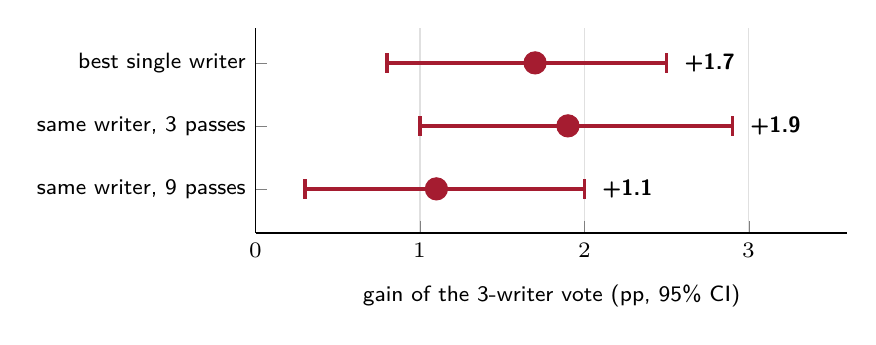
\begin{tikzpicture}
  \begin{axis}[
      width=0.62\linewidth, height=2.6cm, scale only axis,
      xmin=0, xmax=3.6,
      ymin=0.45, ymax=3.7, y dir=reverse,
      ytick={1,2,3},
      yticklabels={{best single writer},{same writer, 3 passes},{same writer, 9 passes}},
      yticklabel style={font=\footnotesize, align=right},
      xtick={0,1,2,3},
      xlabel={gain of the 3-writer vote (pp, 95\% CI)},
      xlabel style={font=\footnotesize},
      tick label style={font=\footnotesize},
      axis x line*=bottom, axis y line*=left,
      xmajorgrids, grid style={black!12},
      error bars/x dir=both, error bars/x explicit,
      error bars/error bar style={line width=1.3pt, hustred},
      error bars/error mark options={rotate=90, mark size=3.5pt, line width=1.3pt, hustred},
    ]
    \addplot[only marks, mark=*, mark size=4pt, hustred] coordinates {
      (1.7,1) += (0.8,0) -= (0.9,0)
      (1.9,2) += (1.0,0) -= (0.9,0)
      (1.1,3) += (0.9,0) -= (0.8,0)
    };
    \node[font=\footnotesize\bfseries, anchor=west, xshift=3pt] at (axis cs:2.5,1) {+1.7};
    \node[font=\footnotesize\bfseries, anchor=west, xshift=3pt] at (axis cs:2.9,2) {+1.9};
    \node[font=\footnotesize\bfseries, anchor=west, xshift=3pt] at (axis cs:2.0,3) {+1.1};
  \end{axis}
\end{tikzpicture}

\vspace{3mm}
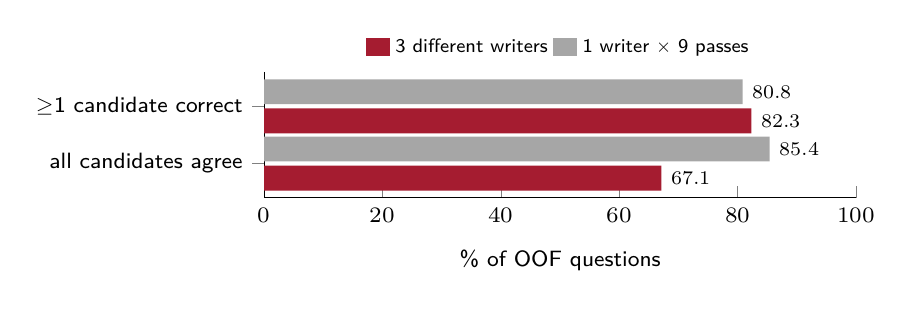
\begin{tikzpicture}
  \begin{axis}[
      width=0.62\linewidth, height=1.6cm, scale only axis,
      xbar=1.5pt, bar width=9pt,
      xmin=0, xmax=100,
      ytick={1,2}, y dir=reverse,
      yticklabels={{$\ge$1 candidate correct},{all candidates agree}},
      yticklabel style={font=\footnotesize, align=right},
      ymin=0.4, ymax=2.6,
      xlabel={\% of OOF questions},
      xlabel style={font=\footnotesize},
      tick label style={font=\footnotesize},
      axis x line*=bottom, axis y line*=left,
      nodes near coords, nodes near coords style={font=\scriptsize\bfseries, /pgf/number format/fixed, /pgf/number format/precision=1},
      legend style={font=\scriptsize, draw=none, fill=none, at={(0.5,1.03)}, anchor=south, legend columns=2},
      legend image code/.code={\draw[#1, draw=none] (0cm,-0.1cm) rectangle (0.3cm,0.12cm);},
    ]
    \addplot[fill=hustred, draw=none] coordinates {(82.3,1) (67.1,2)};
    \addplot[fill=black!35, draw=none] coordinates {(80.8,1) (85.4,2)};
    \legend{3 different writers\quad, 1 writer $\times$ 9 passes}
  \end{axis}
\end{tikzpicture}
\end{center}

  \notepar{Different writers agree less, but hold a correct program more often. Comparisons with one writer's passes are post hoc.}
}

\headerbox{\secno{7}Images help; extra images hurt}{name=img,column=2,below=system,above=errhead}{
  \begin{compactitem}
    \item Removing all images: \textbf{$-$23.3\pp} (public set).
    \item Blanking chart images on 678 OOF chart questions: \textbf{$-$13.4\pp}.
    \item On 1047 OOF questions whose gold reads \emph{no} chart, blanking the images (transcripts kept): \textbf{+1.72\pp} [0.74, 2.73] {\color{muted}(uses the gold; not resolved on the public set)}.
  \end{compactitem}

  \smallskip
  A likely cause is a train/inference mismatch:
  \begin{center}% Train/inference mismatch of the image policy (Sec. 7 of the paper).
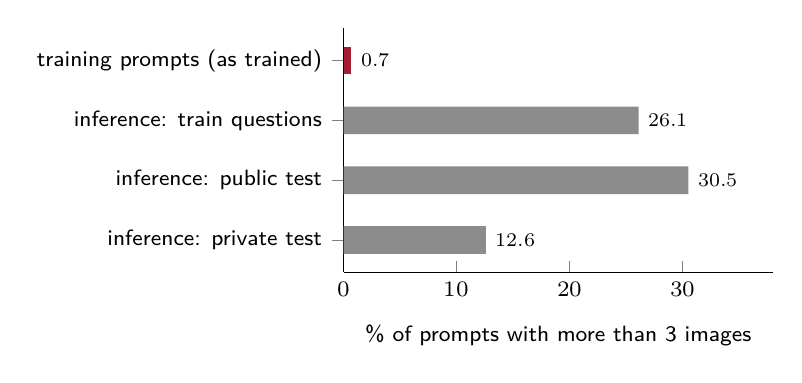
\begin{tikzpicture}
  \begin{axis}[
      width=0.45\linewidth, height=3.1cm, scale only axis,
      xbar, bar width=10pt, bar shift=0pt,
      xmin=0, xmax=38,
      ytick={1,...,4}, y dir=reverse,
      yticklabels={{training prompts (as trained)},{inference: train questions},{inference: public test},{inference: private test}},
      yticklabel style={font=\footnotesize, align=right},
      enlarge y limits=0.18,
      xlabel={\% of prompts with more than 3 images},
      xlabel style={font=\footnotesize},
      tick label style={font=\footnotesize},
      axis x line*=bottom, axis y line*=left,
      nodes near coords, nodes near coords style={font=\scriptsize\bfseries, /pgf/number format/fixed, /pgf/number format/precision=1},
    ]
    \addplot[fill=accent, draw=none] coordinates {(0.7,1)};
    \addplot[fill=black!45, draw=none] coordinates {(26.1,2) (30.5,3) (12.6,4)};
  \end{axis}
\end{tikzpicture}
\end{center}
  \notepar{\textbf{Next step:} train with the inference-time image policy.}
}

\headerbox{\secno{9}Structure and inventory oracles}{name=oracle,column=0,below=errhead,above=bottom}{
  A pre-specified factorial on 1725 OOF questions gives the writer the gold \emph{structure} (operators and \texttt{\#k} dataflow), the gold \emph{inventory} (argument strings), or both.

  \begin{center}% Pre-specified oracle factorial (Fig. 3 of the paper), redrawn.
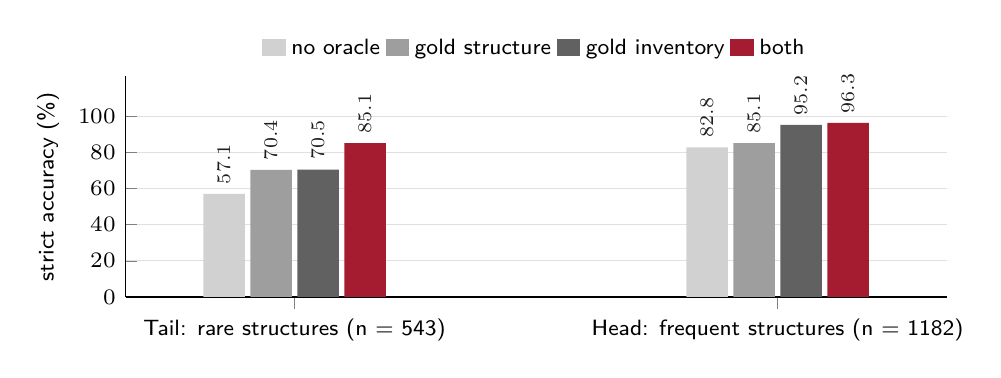
\begin{tikzpicture}
  \begin{axis}[
      width=0.86\linewidth, height=2.8cm, scale only axis,
      ybar=2pt, bar width=15pt,
      ymin=0, ymax=122, ytick={0,20,...,100},
      symbolic x coords={Tail,Head}, xtick=data,
      xticklabels={{Tail: rare structures (n = 543)},{Head: frequent structures (n = 1182)}},
      enlarge x limits=0.35,
      ylabel={strict accuracy (\%)},
      ylabel style={font=\footnotesize},
      tick label style={font=\footnotesize},
      axis x line*=bottom, axis y line*=left,
      ymajorgrids, grid style={black!12},
      nodes near coords, nodes near coords style={font=\scriptsize, rotate=90, anchor=west, color=ink, /pgf/number format/fixed, /pgf/number format/precision=1},
      legend style={font=\footnotesize, draw=none, fill=none, at={(0.5,1.03)}, anchor=south, legend columns=4},
      legend image code/.code={\draw[#1, draw=none] (0cm,-0.1cm) rectangle (0.3cm,0.12cm);},
    ]
    \addplot[fill=black!18, draw=none]   coordinates {(Tail,57.09) (Head,82.83)};
    \addplot[fill=black!38, draw=none]   coordinates {(Tail,70.35) (Head,85.11)};
    \addplot[fill=black!62, draw=none] coordinates {(Tail,70.53) (Head,95.18)};
    \addplot[fill=hustred, draw=none]    coordinates {(Tail,85.08) (Head,96.28)};
    \legend{no oracle, gold structure, gold inventory, both}
  \end{axis}
\end{tikzpicture}
\end{center}

  \notepar{Inventory +12.70\pp, structure +5.74\pp; both 92.75\% (upper bounds). Chance-matched control (1389 q.): lead +8.4 $\to$ +2.8\pp, inconclusive.}
}

\headerbox{\secno{10}Right value, wrong form}{name=form,column=1,below=errhead,above=bottom}{
  \textbf{161 of 435} strict OOF errors (37\%, approximate) execute to the gold value. Many may reflect the Vietnamese presentation of the data: diacritic labels and \emph{triệu / tỷ} scales.

  \begin{center}% Value-equal strict errors of the OOF writers (Sec. 7, Table 14 of the paper).
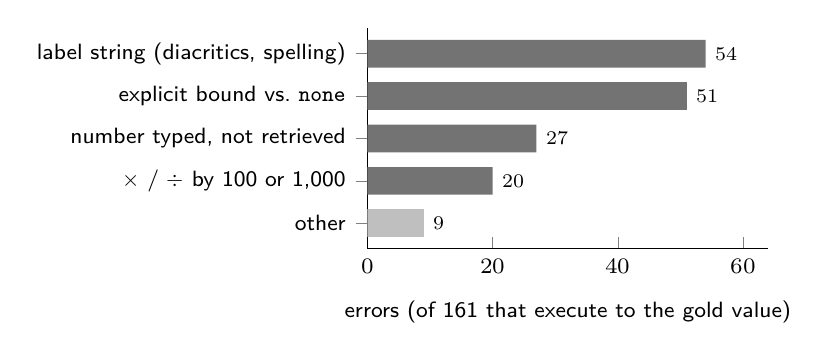
\begin{tikzpicture}
  \begin{axis}[
      width=0.42\linewidth, height=2.8cm, scale only axis,
      xbar, bar width=10pt, bar shift=0pt,
      xmin=0, xmax=64,
      ytick={1,...,5}, y dir=reverse,
      yticklabels={{label string (diacritics, spelling)},{explicit bound vs.\ \texttt{none}},{number typed, not retrieved},{$\times$ / $\div$ by 100 or 1,000},{other}},
      yticklabel style={font=\footnotesize, align=right},
      enlarge y limits=0.15,
      xlabel={errors (of 161 that execute to the gold value)},
      xlabel style={font=\footnotesize},
      tick label style={font=\footnotesize},
      axis x line*=bottom, axis y line*=left,
      nodes near coords, nodes near coords style={font=\scriptsize\bfseries},
    ]
    \addplot[fill=black!55, draw=none] coordinates {(54,1) (51,2) (27,3) (20,4)};
    \addplot[fill=black!25, draw=none] coordinates {(9,5)};
  \end{axis}
\end{tikzpicture}
\end{center}

  \notepar{Picking the gold form among a writer's own samples would reach 77.62\% (from 74.78\%), yet a convention model trained to make that choice changed accuracy by $-$0.17\pp.}
}

\headerbox{\secno{11}Conclusion}{name=concl,column=2,below=errhead}{
  \begin{compactitem}
    \item 26 LoRA-tuned 4B writers ranked \textbf{first of 9} under the 8B limit.
    \item \textbf{Writers that differ} beat more passes of one writer.
    \item Single-writer errors \textbf{begin early}, are \textbf{shared}, and resisted every remedy we tried.
    \item Code, adapters and data went to the organisers; a vote replay reproduces the submissions exactly (retrained adapters: 30~of~980 differ).
  \end{compactitem}
}

\headerbox{References}{name=refs,column=2,below=concl,above=bottom}{
  \scriptsize\color{muted}\raggedright
  \setlength{\parskip}{1.5pt}
  Bai et al.\ 2025. Qwen3-VL technical report. arXiv:2511.21631.\par
  Cameron et al.\ 2008. Bootstrap-based improvements for inference with clustered errors. \mbox{\emph{REStat}}.\par
  Hu et al.\ 2022. LoRA: low-rank adaptation of large language models. \emph{ICLR}.\par
  Kwon et al.\ 2023. PagedAttention (vLLM). \emph{SOSP}.\par
  Qwen Team 2026. Qwen3.5: towards native multimodal agents. Model card.\par
  Wang et al.\ 2023. Self-consistency improves chain of thought reasoning. \emph{ICLR}.\par
  {\tiny\itshape Thanks to the VLSP consortium for data, platform and rulings. Poster examples are constructed.}
}

\end{poster}
\end{document}
